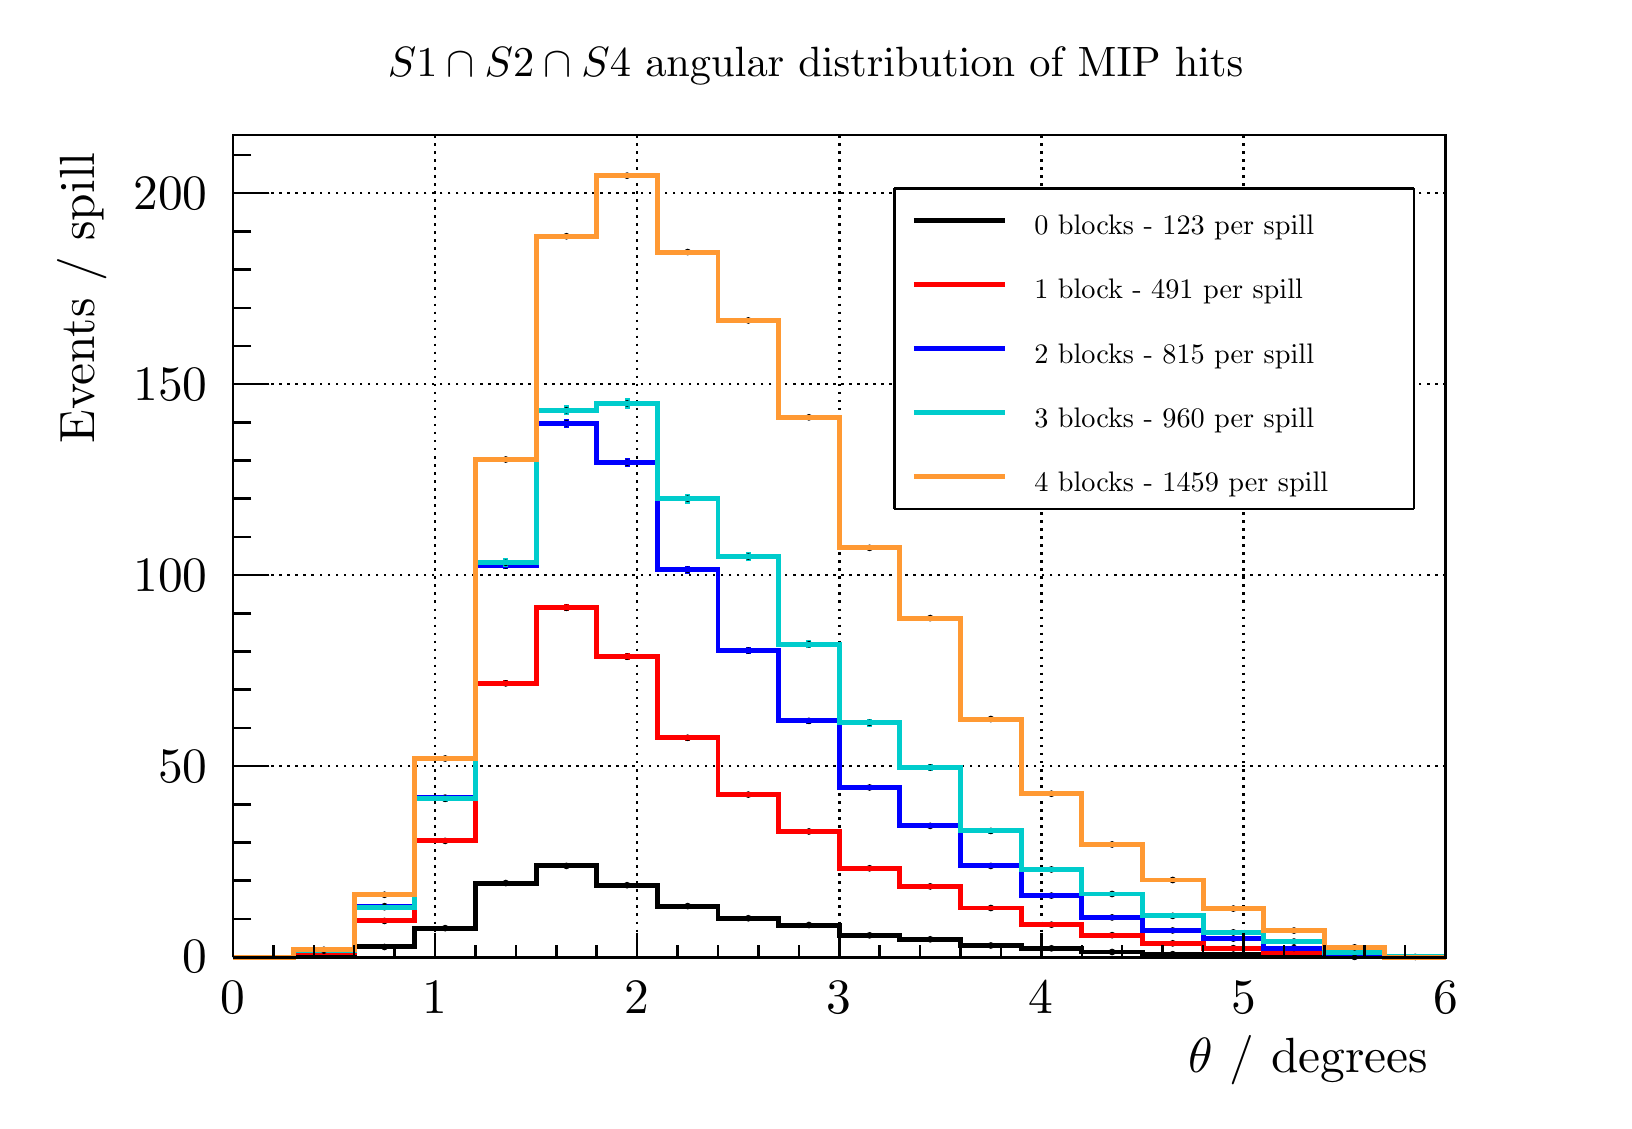
\begin{tikzpicture}
\pgfdeclareplotmark{cross} {
\pgfpathmoveto{\pgfpoint{-0.3\pgfplotmarksize}{\pgfplotmarksize}}
\pgfpathlineto{\pgfpoint{+0.3\pgfplotmarksize}{\pgfplotmarksize}}
\pgfpathlineto{\pgfpoint{+0.3\pgfplotmarksize}{0.3\pgfplotmarksize}}
\pgfpathlineto{\pgfpoint{+1\pgfplotmarksize}{0.3\pgfplotmarksize}}
\pgfpathlineto{\pgfpoint{+1\pgfplotmarksize}{-0.3\pgfplotmarksize}}
\pgfpathlineto{\pgfpoint{+0.3\pgfplotmarksize}{-0.3\pgfplotmarksize}}
\pgfpathlineto{\pgfpoint{+0.3\pgfplotmarksize}{-1.\pgfplotmarksize}}
\pgfpathlineto{\pgfpoint{-0.3\pgfplotmarksize}{-1.\pgfplotmarksize}}
\pgfpathlineto{\pgfpoint{-0.3\pgfplotmarksize}{-0.3\pgfplotmarksize}}
\pgfpathlineto{\pgfpoint{-1.\pgfplotmarksize}{-0.3\pgfplotmarksize}}
\pgfpathlineto{\pgfpoint{-1.\pgfplotmarksize}{0.3\pgfplotmarksize}}
\pgfpathlineto{\pgfpoint{-0.3\pgfplotmarksize}{0.3\pgfplotmarksize}}
\pgfpathclose
\pgfusepathqstroke
}
\pgfdeclareplotmark{cross*} {
\pgfpathmoveto{\pgfpoint{-0.3\pgfplotmarksize}{\pgfplotmarksize}}
\pgfpathlineto{\pgfpoint{+0.3\pgfplotmarksize}{\pgfplotmarksize}}
\pgfpathlineto{\pgfpoint{+0.3\pgfplotmarksize}{0.3\pgfplotmarksize}}
\pgfpathlineto{\pgfpoint{+1\pgfplotmarksize}{0.3\pgfplotmarksize}}
\pgfpathlineto{\pgfpoint{+1\pgfplotmarksize}{-0.3\pgfplotmarksize}}
\pgfpathlineto{\pgfpoint{+0.3\pgfplotmarksize}{-0.3\pgfplotmarksize}}
\pgfpathlineto{\pgfpoint{+0.3\pgfplotmarksize}{-1.\pgfplotmarksize}}
\pgfpathlineto{\pgfpoint{-0.3\pgfplotmarksize}{-1.\pgfplotmarksize}}
\pgfpathlineto{\pgfpoint{-0.3\pgfplotmarksize}{-0.3\pgfplotmarksize}}
\pgfpathlineto{\pgfpoint{-1.\pgfplotmarksize}{-0.3\pgfplotmarksize}}
\pgfpathlineto{\pgfpoint{-1.\pgfplotmarksize}{0.3\pgfplotmarksize}}
\pgfpathlineto{\pgfpoint{-0.3\pgfplotmarksize}{0.3\pgfplotmarksize}}
\pgfpathclose
\pgfusepathqfillstroke
}
\pgfdeclareplotmark{newstar} {
\pgfpathmoveto{\pgfqpoint{0pt}{\pgfplotmarksize}}
\pgfpathlineto{\pgfqpointpolar{44}{0.5\pgfplotmarksize}}
\pgfpathlineto{\pgfqpointpolar{18}{\pgfplotmarksize}}
\pgfpathlineto{\pgfqpointpolar{-20}{0.5\pgfplotmarksize}}
\pgfpathlineto{\pgfqpointpolar{-54}{\pgfplotmarksize}}
\pgfpathlineto{\pgfqpointpolar{-90}{0.5\pgfplotmarksize}}
\pgfpathlineto{\pgfqpointpolar{234}{\pgfplotmarksize}}
\pgfpathlineto{\pgfqpointpolar{198}{0.5\pgfplotmarksize}}
\pgfpathlineto{\pgfqpointpolar{162}{\pgfplotmarksize}}
\pgfpathlineto{\pgfqpointpolar{134}{0.5\pgfplotmarksize}}
\pgfpathclose
\pgfusepathqstroke
}
\pgfdeclareplotmark{newstar*} {
\pgfpathmoveto{\pgfqpoint{0pt}{\pgfplotmarksize}}
\pgfpathlineto{\pgfqpointpolar{44}{0.5\pgfplotmarksize}}
\pgfpathlineto{\pgfqpointpolar{18}{\pgfplotmarksize}}
\pgfpathlineto{\pgfqpointpolar{-20}{0.5\pgfplotmarksize}}
\pgfpathlineto{\pgfqpointpolar{-54}{\pgfplotmarksize}}
\pgfpathlineto{\pgfqpointpolar{-90}{0.5\pgfplotmarksize}}
\pgfpathlineto{\pgfqpointpolar{234}{\pgfplotmarksize}}
\pgfpathlineto{\pgfqpointpolar{198}{0.5\pgfplotmarksize}}
\pgfpathlineto{\pgfqpointpolar{162}{\pgfplotmarksize}}
\pgfpathlineto{\pgfqpointpolar{134}{0.5\pgfplotmarksize}}
\pgfpathclose
\pgfusepathqfillstroke
}
\definecolor{c}{rgb}{1,1,1};
\draw [color=c, fill=c] (0,0) rectangle (20,13.5632);
\draw [color=c, fill=c] (2.6,1.76322) rectangle (18,12.2069);
\definecolor{c}{rgb}{0,0,0};
\draw [c,line width=0.9] (2.6,1.76322) -- (2.6,12.2069) -- (18,12.2069) -- (18,1.76322) -- (2.6,1.76322);
\definecolor{c}{rgb}{1,1,1};
\draw [color=c, fill=c] (2.6,1.76322) rectangle (18,12.2069);
\definecolor{c}{rgb}{0,0,0};
\draw [c,line width=0.9] (2.6,1.76322) -- (2.6,12.2069) -- (18,12.2069) -- (18,1.76322) -- (2.6,1.76322);
\draw [c,line width=0.9] (2.6,1.76322) -- (18,1.76322);
\draw [c,dotted,line width=0.9] (2.6,12.2069) -- (2.6,1.76322);
\draw [c,dotted,line width=0.9] (5.16667,12.2069) -- (5.16667,1.76322);
\draw [c,dotted,line width=0.9] (7.73333,12.2069) -- (7.73333,1.76322);
\draw [c,dotted,line width=0.9] (10.3,12.2069) -- (10.3,1.76322);
\draw [c,dotted,line width=0.9] (12.8667,12.2069) -- (12.8667,1.76322);
\draw [c,dotted,line width=0.9] (15.4333,12.2069) -- (15.4333,1.76322);
\draw [c,dotted,line width=0.9] (18,12.2069) -- (18,1.76322);
\draw [c,line width=0.9] (2.6,1.76322) -- (2.6,12.2069);
\draw [c,dotted,line width=0.9] (18,1.76744) -- (2.6,1.76744);
\draw [c,dotted,line width=0.9] (18,4.19259) -- (2.6,4.19259);
\draw [c,dotted,line width=0.9] (18,6.61774) -- (2.6,6.61774);
\draw [c,dotted,line width=0.9] (18,9.04289) -- (2.6,9.04289);
\draw [c,dotted,line width=0.9] (18,11.468) -- (2.6,11.468);
\draw [c,dotted,line width=0.9] (18,1.76744) -- (2.6,1.76744);
\draw [c,dotted,line width=0.9] (18,11.468) -- (2.6,11.468);
\definecolor{c}{rgb}{0,0,0.6};
\draw [c,line width=0.9] (2.6,1.76744) -- (3.37,1.76744) -- (3.37,1.76744) -- (4.14,1.76744) -- (4.14,1.76744) -- (4.91,1.76744) -- (4.91,1.76744) -- (5.68,1.76744) -- (5.68,1.76744) -- (6.45,1.76744) -- (6.45,1.76744) -- (7.22,1.76744) --
 (7.22,1.76744) -- (7.99,1.76744) -- (7.99,1.76744) -- (8.76,1.76744) -- (8.76,1.76744) -- (9.53,1.76744) -- (9.53,1.76744) -- (10.3,1.76744) -- (10.3,1.76744) -- (11.07,1.76744) -- (11.07,1.76744) -- (11.84,1.76744) -- (11.84,1.76744) --
 (12.61,1.76744) -- (12.61,1.76744) -- (13.38,1.76744) -- (13.38,1.76744) -- (14.15,1.76744) -- (14.15,1.76744) -- (14.92,1.76744) -- (14.92,1.76744) -- (15.69,1.76744) -- (15.69,1.76744) -- (16.46,1.76744) -- (16.46,1.76744) -- (17.23,1.76744) --
 (17.23,1.76744) -- (18,1.76744);
\definecolor{c}{rgb}{0,0,0};
\draw [c,line width=0.9] (2.6,1.76322) -- (18,1.76322);
\draw [anchor= east] (18,0.461149) node[scale=1.78699, color=c, rotate=0]{$\theta$ / degrees};
\draw [c,line width=0.9] (2.6,2.07653) -- (2.6,1.76322);
\draw [c,line width=0.9] (3.11333,1.91987) -- (3.11333,1.76322);
\draw [c,line width=0.9] (3.62667,1.91987) -- (3.62667,1.76322);
\draw [c,line width=0.9] (4.14,1.91987) -- (4.14,1.76322);
\draw [c,line width=0.9] (4.65333,1.91987) -- (4.65333,1.76322);
\draw [c,line width=0.9] (5.16667,2.07653) -- (5.16667,1.76322);
\draw [c,line width=0.9] (5.68,1.91987) -- (5.68,1.76322);
\draw [c,line width=0.9] (6.19333,1.91987) -- (6.19333,1.76322);
\draw [c,line width=0.9] (6.70667,1.91987) -- (6.70667,1.76322);
\draw [c,line width=0.9] (7.22,1.91987) -- (7.22,1.76322);
\draw [c,line width=0.9] (7.73333,2.07653) -- (7.73333,1.76322);
\draw [c,line width=0.9] (8.24667,1.91987) -- (8.24667,1.76322);
\draw [c,line width=0.9] (8.76,1.91987) -- (8.76,1.76322);
\draw [c,line width=0.9] (9.27333,1.91987) -- (9.27333,1.76322);
\draw [c,line width=0.9] (9.78667,1.91987) -- (9.78667,1.76322);
\draw [c,line width=0.9] (10.3,2.07653) -- (10.3,1.76322);
\draw [c,line width=0.9] (10.8133,1.91987) -- (10.8133,1.76322);
\draw [c,line width=0.9] (11.3267,1.91987) -- (11.3267,1.76322);
\draw [c,line width=0.9] (11.84,1.91987) -- (11.84,1.76322);
\draw [c,line width=0.9] (12.3533,1.91987) -- (12.3533,1.76322);
\draw [c,line width=0.9] (12.8667,2.07653) -- (12.8667,1.76322);
\draw [c,line width=0.9] (13.38,1.91987) -- (13.38,1.76322);
\draw [c,line width=0.9] (13.8933,1.91987) -- (13.8933,1.76322);
\draw [c,line width=0.9] (14.4067,1.91987) -- (14.4067,1.76322);
\draw [c,line width=0.9] (14.92,1.91987) -- (14.92,1.76322);
\draw [c,line width=0.9] (15.4333,2.07653) -- (15.4333,1.76322);
\draw [c,line width=0.9] (15.9467,1.91987) -- (15.9467,1.76322);
\draw [c,line width=0.9] (16.46,1.91987) -- (16.46,1.76322);
\draw [c,line width=0.9] (16.9733,1.91987) -- (16.9733,1.76322);
\draw [c,line width=0.9] (17.4867,1.91987) -- (17.4867,1.76322);
\draw [c,line width=0.9] (18,2.07653) -- (18,1.76322);
\draw [anchor=base] (2.6,1.04437) node[scale=1.78699, color=c, rotate=0]{0};
\draw [anchor=base] (5.16667,1.04437) node[scale=1.78699, color=c, rotate=0]{1};
\draw [anchor=base] (7.73333,1.04437) node[scale=1.78699, color=c, rotate=0]{2};
\draw [anchor=base] (10.3,1.04437) node[scale=1.78699, color=c, rotate=0]{3};
\draw [anchor=base] (12.8667,1.04437) node[scale=1.78699, color=c, rotate=0]{4};
\draw [anchor=base] (15.4333,1.04437) node[scale=1.78699, color=c, rotate=0]{5};
\draw [anchor=base] (18,1.04437) node[scale=1.78699, color=c, rotate=0]{6};
\draw [c,line width=0.9] (2.6,1.76322) -- (2.6,12.2069);
\draw [anchor= east] (0.68,12.2069) node[scale=1.78699, color=c, rotate=90]{ Events / spill};
\draw [c,line width=0.9] (3.062,1.76744) -- (2.6,1.76744);
\draw [c,line width=0.9] (2.831,2.25247) -- (2.6,2.25247);
\draw [c,line width=0.9] (2.831,2.7375) -- (2.6,2.7375);
\draw [c,line width=0.9] (2.831,3.22253) -- (2.6,3.22253);
\draw [c,line width=0.9] (2.831,3.70756) -- (2.6,3.70756);
\draw [c,line width=0.9] (3.062,4.19259) -- (2.6,4.19259);
\draw [c,line width=0.9] (2.831,4.67762) -- (2.6,4.67762);
\draw [c,line width=0.9] (2.831,5.16265) -- (2.6,5.16265);
\draw [c,line width=0.9] (2.831,5.64768) -- (2.6,5.64768);
\draw [c,line width=0.9] (2.831,6.13271) -- (2.6,6.13271);
\draw [c,line width=0.9] (3.062,6.61774) -- (2.6,6.61774);
\draw [c,line width=0.9] (2.831,7.10277) -- (2.6,7.10277);
\draw [c,line width=0.9] (2.831,7.5878) -- (2.6,7.5878);
\draw [c,line width=0.9] (2.831,8.07283) -- (2.6,8.07283);
\draw [c,line width=0.9] (2.831,8.55786) -- (2.6,8.55786);
\draw [c,line width=0.9] (3.062,9.04289) -- (2.6,9.04289);
\draw [c,line width=0.9] (2.831,9.52792) -- (2.6,9.52792);
\draw [c,line width=0.9] (2.831,10.0129) -- (2.6,10.0129);
\draw [c,line width=0.9] (2.831,10.498) -- (2.6,10.498);
\draw [c,line width=0.9] (2.831,10.983) -- (2.6,10.983);
\draw [c,line width=0.9] (3.062,11.468) -- (2.6,11.468);
\draw [c,line width=0.9] (3.062,1.76744) -- (2.6,1.76744);
\draw [c,line width=0.9] (3.062,11.468) -- (2.6,11.468);
\draw [c,line width=0.9] (2.831,11.9531) -- (2.6,11.9531);
\draw [anchor= east] (2.5,1.76744) node[scale=1.78699, color=c, rotate=0]{0};
\draw [anchor= east] (2.5,4.19259) node[scale=1.78699, color=c, rotate=0]{50};
\draw [anchor= east] (2.5,6.61774) node[scale=1.78699, color=c, rotate=0]{100};
\draw [anchor= east] (2.5,9.04289) node[scale=1.78699, color=c, rotate=0]{150};
\draw [anchor= east] (2.5,11.468) node[scale=1.78699, color=c, rotate=0]{200};
\draw [c,line width=1.8] (3.755,1.78983) -- (3.755,1.79436);
\draw [c,line width=1.8] (3.755,1.79436) -- (3.755,1.79889);
\foreach \P in {(3.755,1.79436)}{\draw[mark options={color=c,fill=c},mark size=2.402402pt,mark=*,mark size=1pt] plot coordinates {\P};}
\draw [c,line width=1.8] (4.525,1.88561) -- (4.525,1.89499);
\draw [c,line width=1.8] (4.525,1.89499) -- (4.525,1.90437);
\foreach \P in {(4.525,1.89499)}{\draw[mark options={color=c,fill=c},mark size=2.402402pt,mark=*,mark size=1pt] plot coordinates {\P};}
\draw [c,line width=1.8] (5.295,2.11945) -- (5.295,2.13418);
\draw [c,line width=1.8] (5.295,2.13418) -- (5.295,2.14891);
\foreach \P in {(5.295,2.13418)}{\draw[mark options={color=c,fill=c},mark size=2.402402pt,mark=*,mark size=1pt] plot coordinates {\P};}
\draw [c,line width=1.8] (6.065,2.68461) -- (6.065,2.70679);
\draw [c,line width=1.8] (6.065,2.70679) -- (6.065,2.72898);
\foreach \P in {(6.065,2.70679)}{\draw[mark options={color=c,fill=c},mark size=2.402402pt,mark=*,mark size=1pt] plot coordinates {\P};}
\draw [c,line width=1.8] (6.835,2.9007) -- (6.835,2.92469);
\draw [c,line width=1.8] (6.835,2.92469) -- (6.835,2.94868);
\foreach \P in {(6.835,2.92469)}{\draw[mark options={color=c,fill=c},mark size=2.402402pt,mark=*,mark size=1pt] plot coordinates {\P};}
\draw [c,line width=1.8] (7.605,2.65802) -- (7.605,2.67959);
\draw [c,line width=1.8] (7.605,2.67959) -- (7.605,2.70116);
\foreach \P in {(7.605,2.67959)}{\draw[mark options={color=c,fill=c},mark size=2.402402pt,mark=*,mark size=1pt] plot coordinates {\P};}
\draw [c,line width=1.8] (8.375,2.39545) -- (8.375,2.41427);
\draw [c,line width=1.8] (8.375,2.41427) -- (8.375,2.4331);
\foreach \P in {(8.375,2.41427)}{\draw[mark options={color=c,fill=c},mark size=2.402402pt,mark=*,mark size=1pt] plot coordinates {\P};}
\draw [c,line width=1.8] (9.145,2.24317) -- (9.145,2.25985);
\draw [c,line width=1.8] (9.145,2.25985) -- (9.145,2.27654);
\foreach \P in {(9.145,2.25985)}{\draw[mark options={color=c,fill=c},mark size=2.402402pt,mark=*,mark size=1pt] plot coordinates {\P};}
\draw [c,line width=1.8] (9.915,2.15841) -- (9.915,2.17379);
\draw [c,line width=1.8] (9.915,2.17379) -- (9.915,2.18916);
\foreach \P in {(9.915,2.17379)}{\draw[mark options={color=c,fill=c},mark size=2.402402pt,mark=*,mark size=1pt] plot coordinates {\P};}
\draw [c,line width=1.8] (10.685,2.02998) -- (10.685,2.04288);
\draw [c,line width=1.8] (10.685,2.04288) -- (10.685,2.05579);
\foreach \P in {(10.685,2.04288)}{\draw[mark options={color=c,fill=c},mark size=2.402402pt,mark=*,mark size=1pt] plot coordinates {\P};}
\draw [c,line width=1.8] (11.455,1.9807) -- (11.455,1.99236);
\draw [c,line width=1.8] (11.455,1.99236) -- (11.455,2.00403);
\foreach \P in {(11.455,1.99236)}{\draw[mark options={color=c,fill=c},mark size=2.402402pt,mark=*,mark size=1pt] plot coordinates {\P};}
\draw [c,line width=1.8] (12.225,1.90443) -- (12.225,1.91395);
\draw [c,line width=1.8] (12.225,1.91395) -- (12.225,1.92347);
\foreach \P in {(12.225,1.91395)}{\draw[mark options={color=c,fill=c},mark size=2.402402pt,mark=*,mark size=1pt] plot coordinates {\P};}
\draw [c,line width=1.8] (12.995,1.86923) -- (12.995,1.87784);
\draw [c,line width=1.8] (12.995,1.87784) -- (12.995,1.88644);
\foreach \P in {(12.995,1.87784)}{\draw[mark options={color=c,fill=c},mark size=2.402402pt,mark=*,mark size=1pt] plot coordinates {\P};}
\draw [c,line width=1.8] (13.765,1.82465) -- (13.765,1.83133);
\draw [c,line width=1.8] (13.765,1.83133) -- (13.765,1.83801);
\foreach \P in {(13.765,1.83133)}{\draw[mark options={color=c,fill=c},mark size=2.402402pt,mark=*,mark size=1pt] plot coordinates {\P};}
\draw [c,line width=1.8] (14.535,1.79842) -- (14.535,1.80368);
\draw [c,line width=1.8] (14.535,1.80368) -- (14.535,1.80894);
\foreach \P in {(14.535,1.80368)}{\draw[mark options={color=c,fill=c},mark size=2.402402pt,mark=*,mark size=1pt] plot coordinates {\P};}
\draw [c,line width=1.8] (15.305,1.79286) -- (15.305,1.79794);
\draw [c,line width=1.8] (15.305,1.79794) -- (15.305,1.80301);
\foreach \P in {(15.305,1.79794)}{\draw[mark options={color=c,fill=c},mark size=2.402402pt,mark=*,mark size=1pt] plot coordinates {\P};}
\draw [c,line width=1.8] (16.075,1.7812) -- (16.075,1.78518);
\draw [c,line width=1.8] (16.075,1.78518) -- (16.075,1.78916);
\foreach \P in {(16.075,1.78518)}{\draw[mark options={color=c,fill=c},mark size=2.402402pt,mark=*,mark size=1pt] plot coordinates {\P};}
\draw [c,line width=1.8] (16.845,1.76709) -- (16.845,1.76925);
\draw [c,line width=1.8] (16.845,1.76925) -- (16.845,1.77141);
\foreach \P in {(16.845,1.76925)}{\draw[mark options={color=c,fill=c},mark size=2.402402pt,mark=*,mark size=1pt] plot coordinates {\P};}
\draw [c,line width=1.8] (2.6,1.76744) -- (3.37,1.76744) -- (3.37,1.79436) -- (4.14,1.79436) -- (4.14,1.89499) -- (4.91,1.89499) -- (4.91,2.13418) -- (5.68,2.13418) -- (5.68,2.70679) -- (6.45,2.70679) -- (6.45,2.92469) -- (7.22,2.92469) --
 (7.22,2.67959) -- (7.99,2.67959) -- (7.99,2.41427) -- (8.76,2.41427) -- (8.76,2.25985) -- (9.53,2.25985) -- (9.53,2.17379) -- (10.3,2.17379) -- (10.3,2.04288) -- (11.07,2.04288) -- (11.07,1.99236) -- (11.84,1.99236) -- (11.84,1.91395) --
 (12.61,1.91395) -- (12.61,1.87784) -- (13.38,1.87784) -- (13.38,1.83133) -- (14.15,1.83133) -- (14.15,1.80368) -- (14.92,1.80368) -- (14.92,1.79794) -- (15.69,1.79794) -- (15.69,1.78518) -- (16.46,1.78518) -- (16.46,1.76925) -- (17.23,1.76925) --
 (17.23,1.76744) -- (18,1.76744);
\definecolor{c}{rgb}{1,0,0};
\draw [c,line width=1.8] (3.755,1.81396) -- (3.755,1.81942);
\draw [c,line width=1.8] (3.755,1.81942) -- (3.755,1.82488);
\definecolor{c}{rgb}{0,0,0};
\foreach \P in {(3.755,1.81942)}{\draw[mark options={color=c,fill=c},mark size=2.402402pt,mark=*,mark size=1pt] plot coordinates {\P};}
\definecolor{c}{rgb}{1,0,0};
\draw [c,line width=1.8] (4.525,2.21057) -- (4.525,2.22581);
\draw [c,line width=1.8] (4.525,2.22581) -- (4.525,2.24106);
\definecolor{c}{rgb}{0,0,0};
\foreach \P in {(4.525,2.22581)}{\draw[mark options={color=c,fill=c},mark size=2.402402pt,mark=*,mark size=1pt] plot coordinates {\P};}
\definecolor{c}{rgb}{1,0,0};
\draw [c,line width=1.8] (5.295,3.21613) -- (5.295,3.24228);
\draw [c,line width=1.8] (5.295,3.24228) -- (5.295,3.26842);
\definecolor{c}{rgb}{0,0,0};
\foreach \P in {(5.295,3.24228)}{\draw[mark options={color=c,fill=c},mark size=2.402402pt,mark=*,mark size=1pt] plot coordinates {\P};}
\definecolor{c}{rgb}{1,0,0};
\draw [c,line width=1.8] (6.065,5.20308) -- (6.065,5.24251);
\draw [c,line width=1.8] (6.065,5.24251) -- (6.065,5.28193);
\definecolor{c}{rgb}{0,0,0};
\foreach \P in {(6.065,5.24251)}{\draw[mark options={color=c,fill=c},mark size=2.402402pt,mark=*,mark size=1pt] plot coordinates {\P};}
\definecolor{c}{rgb}{1,0,0};
\draw [c,line width=1.8] (6.835,6.15816) -- (6.835,6.20243);
\draw [c,line width=1.8] (6.835,6.20243) -- (6.835,6.24669);
\definecolor{c}{rgb}{0,0,0};
\foreach \P in {(6.835,6.20243)}{\draw[mark options={color=c,fill=c},mark size=2.402402pt,mark=*,mark size=1pt] plot coordinates {\P};}
\definecolor{c}{rgb}{1,0,0};
\draw [c,line width=1.8] (7.605,5.5402) -- (7.605,5.58196);
\draw [c,line width=1.8] (7.605,5.58196) -- (7.605,5.62371);
\definecolor{c}{rgb}{0,0,0};
\foreach \P in {(7.605,5.58196)}{\draw[mark options={color=c,fill=c},mark size=2.402402pt,mark=*,mark size=1pt] plot coordinates {\P};}
\definecolor{c}{rgb}{1,0,0};
\draw [c,line width=1.8] (8.375,4.51598) -- (8.375,4.55208);
\draw [c,line width=1.8] (8.375,4.55208) -- (8.375,4.58817);
\definecolor{c}{rgb}{0,0,0};
\foreach \P in {(8.375,4.55208)}{\draw[mark options={color=c,fill=c},mark size=2.402402pt,mark=*,mark size=1pt] plot coordinates {\P};}
\definecolor{c}{rgb}{1,0,0};
\draw [c,line width=1.8] (9.145,3.79835) -- (9.145,3.83014);
\draw [c,line width=1.8] (9.145,3.83014) -- (9.145,3.86192);
\definecolor{c}{rgb}{0,0,0};
\foreach \P in {(9.145,3.83014)}{\draw[mark options={color=c,fill=c},mark size=2.402402pt,mark=*,mark size=1pt] plot coordinates {\P};}
\definecolor{c}{rgb}{1,0,0};
\draw [c,line width=1.8] (9.915,3.33388) -- (9.915,3.36201);
\draw [c,line width=1.8] (9.915,3.36201) -- (9.915,3.39015);
\definecolor{c}{rgb}{0,0,0};
\foreach \P in {(9.915,3.36201)}{\draw[mark options={color=c,fill=c},mark size=2.402402pt,mark=*,mark size=1pt] plot coordinates {\P};}
\definecolor{c}{rgb}{1,0,0};
\draw [c,line width=1.8] (10.685,2.87003) -- (10.685,2.89427);
\draw [c,line width=1.8] (10.685,2.89427) -- (10.685,2.91852);
\definecolor{c}{rgb}{0,0,0};
\foreach \P in {(10.685,2.89427)}{\draw[mark options={color=c,fill=c},mark size=2.402402pt,mark=*,mark size=1pt] plot coordinates {\P};}
\definecolor{c}{rgb}{1,0,0};
\draw [c,line width=1.8] (11.455,2.64248) -- (11.455,2.66431);
\draw [c,line width=1.8] (11.455,2.66431) -- (11.455,2.68613);
\definecolor{c}{rgb}{0,0,0};
\foreach \P in {(11.455,2.66431)}{\draw[mark options={color=c,fill=c},mark size=2.402402pt,mark=*,mark size=1pt] plot coordinates {\P};}
\definecolor{c}{rgb}{1,0,0};
\draw [c,line width=1.8] (12.225,2.37137) -- (12.225,2.38992);
\draw [c,line width=1.8] (12.225,2.38992) -- (12.225,2.40847);
\definecolor{c}{rgb}{0,0,0};
\foreach \P in {(12.225,2.38992)}{\draw[mark options={color=c,fill=c},mark size=2.402402pt,mark=*,mark size=1pt] plot coordinates {\P};}
\definecolor{c}{rgb}{1,0,0};
\draw [c,line width=1.8] (12.995,2.16257) -- (12.995,2.17821);
\draw [c,line width=1.8] (12.995,2.17821) -- (12.995,2.19386);
\definecolor{c}{rgb}{0,0,0};
\foreach \P in {(12.995,2.17821)}{\draw[mark options={color=c,fill=c},mark size=2.402402pt,mark=*,mark size=1pt] plot coordinates {\P};}
\definecolor{c}{rgb}{1,0,0};
\draw [c,line width=1.8] (13.765,2.0315) -- (13.765,2.04493);
\draw [c,line width=1.8] (13.765,2.04493) -- (13.765,2.05836);
\definecolor{c}{rgb}{0,0,0};
\foreach \P in {(13.765,2.04493)}{\draw[mark options={color=c,fill=c},mark size=2.402402pt,mark=*,mark size=1pt] plot coordinates {\P};}
\definecolor{c}{rgb}{1,0,0};
\draw [c,line width=1.8] (14.535,1.93052) -- (14.535,1.94126);
\draw [c,line width=1.8] (14.535,1.94126) -- (14.535,1.952);
\definecolor{c}{rgb}{0,0,0};
\foreach \P in {(14.535,1.94126)}{\draw[mark options={color=c,fill=c},mark size=2.402402pt,mark=*,mark size=1pt] plot coordinates {\P};}
\definecolor{c}{rgb}{1,0,0};
\draw [c,line width=1.8] (15.305,1.87034) -- (15.305,1.87956);
\draw [c,line width=1.8] (15.305,1.87956) -- (15.305,1.88878);
\definecolor{c}{rgb}{0,0,0};
\foreach \P in {(15.305,1.87956)}{\draw[mark options={color=c,fill=c},mark size=2.402402pt,mark=*,mark size=1pt] plot coordinates {\P};}
\definecolor{c}{rgb}{1,0,0};
\draw [c,line width=1.8] (16.075,1.82261) -- (16.075,1.8304);
\draw [c,line width=1.8] (16.075,1.8304) -- (16.075,1.8382);
\definecolor{c}{rgb}{0,0,0};
\foreach \P in {(16.075,1.8304)}{\draw[mark options={color=c,fill=c},mark size=2.402402pt,mark=*,mark size=1pt] plot coordinates {\P};}
\definecolor{c}{rgb}{1,0,0};
\draw [c,line width=1.8] (16.845,1.77091) -- (16.845,1.77506);
\draw [c,line width=1.8] (16.845,1.77506) -- (16.845,1.77922);
\definecolor{c}{rgb}{0,0,0};
\foreach \P in {(16.845,1.77506)}{\draw[mark options={color=c,fill=c},mark size=2.402402pt,mark=*,mark size=1pt] plot coordinates {\P};}
\definecolor{c}{rgb}{1,0,0};
\draw [c,line width=1.8] (2.6,1.76744) -- (3.37,1.76744) -- (3.37,1.81942) -- (4.14,1.81942) -- (4.14,2.22581) -- (4.91,2.22581) -- (4.91,3.24228) -- (5.68,3.24228) -- (5.68,5.24251) -- (6.45,5.24251) -- (6.45,6.20243) -- (7.22,6.20243) --
 (7.22,5.58196) -- (7.99,5.58196) -- (7.99,4.55208) -- (8.76,4.55208) -- (8.76,3.83014) -- (9.53,3.83014) -- (9.53,3.36201) -- (10.3,3.36201) -- (10.3,2.89427) -- (11.07,2.89427) -- (11.07,2.66431) -- (11.84,2.66431) -- (11.84,2.38992) --
 (12.61,2.38992) -- (12.61,2.17821) -- (13.38,2.17821) -- (13.38,2.04493) -- (14.15,2.04493) -- (14.15,1.94126) -- (14.92,1.94126) -- (14.92,1.87956) -- (15.69,1.87956) -- (15.69,1.8304) -- (16.46,1.8304) -- (16.46,1.77506) -- (17.23,1.77506) --
 (17.23,1.76744) -- (18,1.76744);
\definecolor{c}{rgb}{0,0,1};
\draw [c,line width=1.8] (3.755,1.84408) -- (3.755,1.85134);
\draw [c,line width=1.8] (3.755,1.85134) -- (3.755,1.8586);
\definecolor{c}{rgb}{0,0,0};
\foreach \P in {(3.755,1.85134)}{\draw[mark options={color=c,fill=c},mark size=2.402402pt,mark=*,mark size=1pt] plot coordinates {\P};}
\definecolor{c}{rgb}{0,0,1};
\draw [c,line width=1.8] (4.525,2.39435) -- (4.525,2.41302);
\draw [c,line width=1.8] (4.525,2.41302) -- (4.525,2.43169);
\definecolor{c}{rgb}{0,0,0};
\foreach \P in {(4.525,2.41302)}{\draw[mark options={color=c,fill=c},mark size=2.402402pt,mark=*,mark size=1pt] plot coordinates {\P};}
\definecolor{c}{rgb}{0,0,1};
\draw [c,line width=1.8] (5.295,3.76008) -- (5.295,3.79169);
\draw [c,line width=1.8] (5.295,3.79169) -- (5.295,3.82329);
\definecolor{c}{rgb}{0,0,0};
\foreach \P in {(5.295,3.79169)}{\draw[mark options={color=c,fill=c},mark size=2.402402pt,mark=*,mark size=1pt] plot coordinates {\P};}
\definecolor{c}{rgb}{0,0,1};
\draw [c,line width=1.8] (6.065,6.68987) -- (6.065,6.73794);
\draw [c,line width=1.8] (6.065,6.73794) -- (6.065,6.78601);
\definecolor{c}{rgb}{0,0,0};
\foreach \P in {(6.065,6.73794)}{\draw[mark options={color=c,fill=c},mark size=2.402402pt,mark=*,mark size=1pt] plot coordinates {\P};}
\definecolor{c}{rgb}{0,0,1};
\draw [c,line width=1.8] (6.835,8.49075) -- (6.835,8.54602);
\draw [c,line width=1.8] (6.835,8.54602) -- (6.835,8.60129);
\definecolor{c}{rgb}{0,0,0};
\foreach \P in {(6.835,8.54602)}{\draw[mark options={color=c,fill=c},mark size=2.402402pt,mark=*,mark size=1pt] plot coordinates {\P};}
\definecolor{c}{rgb}{0,0,1};
\draw [c,line width=1.8] (7.605,7.9918) -- (7.605,8.04532);
\draw [c,line width=1.8] (7.605,8.04532) -- (7.605,8.09884);
\definecolor{c}{rgb}{0,0,0};
\foreach \P in {(7.605,8.04532)}{\draw[mark options={color=c,fill=c},mark size=2.402402pt,mark=*,mark size=1pt] plot coordinates {\P};}
\definecolor{c}{rgb}{0,0,1};
\draw [c,line width=1.8] (8.375,6.63685) -- (8.375,6.68509);
\draw [c,line width=1.8] (8.375,6.68509) -- (8.375,6.73333);
\definecolor{c}{rgb}{0,0,0};
\foreach \P in {(8.375,6.68509)}{\draw[mark options={color=c,fill=c},mark size=2.402402pt,mark=*,mark size=1pt] plot coordinates {\P};}
\definecolor{c}{rgb}{0,0,1};
\draw [c,line width=1.8] (9.145,5.61567) -- (9.145,5.65956);
\draw [c,line width=1.8] (9.145,5.65956) -- (9.145,5.70345);
\definecolor{c}{rgb}{0,0,0};
\foreach \P in {(9.145,5.65956)}{\draw[mark options={color=c,fill=c},mark size=2.402402pt,mark=*,mark size=1pt] plot coordinates {\P};}
\definecolor{c}{rgb}{0,0,1};
\draw [c,line width=1.8] (9.915,4.72777) -- (9.915,4.76661);
\draw [c,line width=1.8] (9.915,4.76661) -- (9.915,4.80545);
\definecolor{c}{rgb}{0,0,0};
\foreach \P in {(9.915,4.76661)}{\draw[mark options={color=c,fill=c},mark size=2.402402pt,mark=*,mark size=1pt] plot coordinates {\P};}
\definecolor{c}{rgb}{0,0,1};
\draw [c,line width=1.8] (10.685,3.88714) -- (10.685,3.92086);
\draw [c,line width=1.8] (10.685,3.92086) -- (10.685,3.95458);
\definecolor{c}{rgb}{0,0,0};
\foreach \P in {(10.685,3.92086)}{\draw[mark options={color=c,fill=c},mark size=2.402402pt,mark=*,mark size=1pt] plot coordinates {\P};}
\definecolor{c}{rgb}{0,0,1};
\draw [c,line width=1.8] (11.455,3.40333) -- (11.455,3.43318);
\draw [c,line width=1.8] (11.455,3.43318) -- (11.455,3.46303);
\definecolor{c}{rgb}{0,0,0};
\foreach \P in {(11.455,3.43318)}{\draw[mark options={color=c,fill=c},mark size=2.402402pt,mark=*,mark size=1pt] plot coordinates {\P};}
\definecolor{c}{rgb}{0,0,1};
\draw [c,line width=1.8] (12.225,2.89917) -- (12.225,2.92452);
\draw [c,line width=1.8] (12.225,2.92452) -- (12.225,2.94987);
\definecolor{c}{rgb}{0,0,0};
\foreach \P in {(12.225,2.92452)}{\draw[mark options={color=c,fill=c},mark size=2.402402pt,mark=*,mark size=1pt] plot coordinates {\P};}
\definecolor{c}{rgb}{0,0,1};
\draw [c,line width=1.8] (12.995,2.52582) -- (12.995,2.54757);
\draw [c,line width=1.8] (12.995,2.54757) -- (12.995,2.56932);
\definecolor{c}{rgb}{0,0,0};
\foreach \P in {(12.995,2.54757)}{\draw[mark options={color=c,fill=c},mark size=2.402402pt,mark=*,mark size=1pt] plot coordinates {\P};}
\definecolor{c}{rgb}{0,0,1};
\draw [c,line width=1.8] (13.765,2.25214) -- (13.765,2.27022);
\draw [c,line width=1.8] (13.765,2.27022) -- (13.765,2.2883);
\definecolor{c}{rgb}{0,0,0};
\foreach \P in {(13.765,2.27022)}{\draw[mark options={color=c,fill=c},mark size=2.402402pt,mark=*,mark size=1pt] plot coordinates {\P};}
\definecolor{c}{rgb}{0,0,1};
\draw [c,line width=1.8] (14.535,2.08946) -- (14.535,2.10492);
\draw [c,line width=1.8] (14.535,2.10492) -- (14.535,2.12039);
\definecolor{c}{rgb}{0,0,0};
\foreach \P in {(14.535,2.10492)}{\draw[mark options={color=c,fill=c},mark size=2.402402pt,mark=*,mark size=1pt] plot coordinates {\P};}
\definecolor{c}{rgb}{0,0,1};
\draw [c,line width=1.8] (15.305,1.98767) -- (15.305,2.00128);
\draw [c,line width=1.8] (15.305,2.00128) -- (15.305,2.01488);
\definecolor{c}{rgb}{0,0,0};
\foreach \P in {(15.305,2.00128)}{\draw[mark options={color=c,fill=c},mark size=2.402402pt,mark=*,mark size=1pt] plot coordinates {\P};}
\definecolor{c}{rgb}{0,0,1};
\draw [c,line width=1.8] (16.075,1.87059) -- (16.075,1.88108);
\draw [c,line width=1.8] (16.075,1.88108) -- (16.075,1.89157);
\definecolor{c}{rgb}{0,0,0};
\foreach \P in {(16.075,1.88108)}{\draw[mark options={color=c,fill=c},mark size=2.402402pt,mark=*,mark size=1pt] plot coordinates {\P};}
\definecolor{c}{rgb}{0,0,1};
\draw [c,line width=1.8] (16.845,1.7943) -- (16.845,1.80135);
\draw [c,line width=1.8] (16.845,1.80135) -- (16.845,1.8084);
\definecolor{c}{rgb}{0,0,0};
\foreach \P in {(16.845,1.80135)}{\draw[mark options={color=c,fill=c},mark size=2.402402pt,mark=*,mark size=1pt] plot coordinates {\P};}
\definecolor{c}{rgb}{0,0,1};
\draw [c,line width=1.8] (2.6,1.76744) -- (3.37,1.76744) -- (3.37,1.85134) -- (4.14,1.85134) -- (4.14,2.41302) -- (4.91,2.41302) -- (4.91,3.79169) -- (5.68,3.79169) -- (5.68,6.73794) -- (6.45,6.73794) -- (6.45,8.54602) -- (7.22,8.54602) --
 (7.22,8.04532) -- (7.99,8.04532) -- (7.99,6.68509) -- (8.76,6.68509) -- (8.76,5.65956) -- (9.53,5.65956) -- (9.53,4.76661) -- (10.3,4.76661) -- (10.3,3.92086) -- (11.07,3.92086) -- (11.07,3.43318) -- (11.84,3.43318) -- (11.84,2.92452) --
 (12.61,2.92452) -- (12.61,2.54757) -- (13.38,2.54757) -- (13.38,2.27022) -- (14.15,2.27022) -- (14.15,2.10492) -- (14.92,2.10492) -- (14.92,2.00128) -- (15.69,2.00128) -- (15.69,1.88108) -- (16.46,1.88108) -- (16.46,1.80135) -- (17.23,1.80135) --
 (17.23,1.76744) -- (18,1.76744);
\definecolor{c}{rgb}{0,0.8,0.8};
\draw [c,line width=1.8] (3.755,1.84134) -- (3.755,1.84959);
\draw [c,line width=1.8] (3.755,1.84959) -- (3.755,1.85784);
\definecolor{c}{rgb}{0,0,0};
\foreach \P in {(3.755,1.84959)}{\draw[mark options={color=c,fill=c},mark size=2.402402pt,mark=*,mark size=1pt] plot coordinates {\P};}
\definecolor{c}{rgb}{0,0.8,0.8};
\draw [c,line width=1.8] (4.525,2.37933) -- (4.525,2.40063);
\draw [c,line width=1.8] (4.525,2.40063) -- (4.525,2.42192);
\definecolor{c}{rgb}{0,0,0};
\foreach \P in {(4.525,2.40063)}{\draw[mark options={color=c,fill=c},mark size=2.402402pt,mark=*,mark size=1pt] plot coordinates {\P};}
\definecolor{c}{rgb}{0,0.8,0.8};
\draw [c,line width=1.8] (5.295,3.74049) -- (5.295,3.77657);
\draw [c,line width=1.8] (5.295,3.77657) -- (5.295,3.81265);
\definecolor{c}{rgb}{0,0,0};
\foreach \P in {(5.295,3.77657)}{\draw[mark options={color=c,fill=c},mark size=2.402402pt,mark=*,mark size=1pt] plot coordinates {\P};}
\definecolor{c}{rgb}{0,0.8,0.8};
\draw [c,line width=1.8] (6.065,6.71858) -- (6.065,6.7739);
\draw [c,line width=1.8] (6.065,6.7739) -- (6.065,6.82921);
\definecolor{c}{rgb}{0,0,0};
\foreach \P in {(6.065,6.7739)}{\draw[mark options={color=c,fill=c},mark size=2.402402pt,mark=*,mark size=1pt] plot coordinates {\P};}
\definecolor{c}{rgb}{0,0.8,0.8};
\draw [c,line width=1.8] (6.835,8.64689) -- (6.835,8.71101);
\draw [c,line width=1.8] (6.835,8.71101) -- (6.835,8.77513);
\definecolor{c}{rgb}{0,0,0};
\foreach \P in {(6.835,8.71101)}{\draw[mark options={color=c,fill=c},mark size=2.402402pt,mark=*,mark size=1pt] plot coordinates {\P};}
\definecolor{c}{rgb}{0,0.8,0.8};
\draw [c,line width=1.8] (7.605,8.73228) -- (7.605,8.79806);
\draw [c,line width=1.8] (7.605,8.79806) -- (7.605,8.86384);
\definecolor{c}{rgb}{0,0,0};
\foreach \P in {(7.605,8.79806)}{\draw[mark options={color=c,fill=c},mark size=2.402402pt,mark=*,mark size=1pt] plot coordinates {\P};}
\definecolor{c}{rgb}{0,0.8,0.8};
\draw [c,line width=1.8] (8.375,7.52703) -- (8.375,7.58837);
\draw [c,line width=1.8] (8.375,7.58837) -- (8.375,7.6497);
\definecolor{c}{rgb}{0,0,0};
\foreach \P in {(8.375,7.58837)}{\draw[mark options={color=c,fill=c},mark size=2.402402pt,mark=*,mark size=1pt] plot coordinates {\P};}
\definecolor{c}{rgb}{0,0.8,0.8};
\draw [c,line width=1.8] (9.145,6.79362) -- (9.145,6.85271);
\draw [c,line width=1.8] (9.145,6.85271) -- (9.145,6.91179);
\definecolor{c}{rgb}{0,0,0};
\foreach \P in {(9.145,6.85271)}{\draw[mark options={color=c,fill=c},mark size=2.402402pt,mark=*,mark size=1pt] plot coordinates {\P};}
\definecolor{c}{rgb}{0,0.8,0.8};
\draw [c,line width=1.8] (9.915,5.68617) -- (9.915,5.73927);
\draw [c,line width=1.8] (9.915,5.73927) -- (9.915,5.79236);
\definecolor{c}{rgb}{0,0,0};
\foreach \P in {(9.915,5.73927)}{\draw[mark options={color=c,fill=c},mark size=2.402402pt,mark=*,mark size=1pt] plot coordinates {\P};}
\definecolor{c}{rgb}{0,0.8,0.8};
\draw [c,line width=1.8] (10.685,4.69497) -- (10.685,4.74204);
\draw [c,line width=1.8] (10.685,4.74204) -- (10.685,4.78911);
\definecolor{c}{rgb}{0,0,0};
\foreach \P in {(10.685,4.74204)}{\draw[mark options={color=c,fill=c},mark size=2.402402pt,mark=*,mark size=1pt] plot coordinates {\P};}
\definecolor{c}{rgb}{0,0.8,0.8};
\draw [c,line width=1.8] (11.455,4.13163) -- (11.455,4.17519);
\draw [c,line width=1.8] (11.455,4.17519) -- (11.455,4.21874);
\definecolor{c}{rgb}{0,0,0};
\foreach \P in {(11.455,4.17519)}{\draw[mark options={color=c,fill=c},mark size=2.402402pt,mark=*,mark size=1pt] plot coordinates {\P};}
\definecolor{c}{rgb}{0,0.8,0.8};
\draw [c,line width=1.8] (12.225,3.33326) -- (12.225,3.36898);
\draw [c,line width=1.8] (12.225,3.36898) -- (12.225,3.4047);
\definecolor{c}{rgb}{0,0,0};
\foreach \P in {(12.225,3.36898)}{\draw[mark options={color=c,fill=c},mark size=2.402402pt,mark=*,mark size=1pt] plot coordinates {\P};}
\definecolor{c}{rgb}{0,0.8,0.8};
\draw [c,line width=1.8] (12.995,2.84872) -- (12.995,2.87968);
\draw [c,line width=1.8] (12.995,2.87968) -- (12.995,2.91065);
\definecolor{c}{rgb}{0,0,0};
\foreach \P in {(12.995,2.87968)}{\draw[mark options={color=c,fill=c},mark size=2.402402pt,mark=*,mark size=1pt] plot coordinates {\P};}
\definecolor{c}{rgb}{0,0.8,0.8};
\draw [c,line width=1.8] (13.765,2.53969) -- (13.765,2.56783);
\draw [c,line width=1.8] (13.765,2.56783) -- (13.765,2.59596);
\definecolor{c}{rgb}{0,0,0};
\foreach \P in {(13.765,2.56783)}{\draw[mark options={color=c,fill=c},mark size=2.402402pt,mark=*,mark size=1pt] plot coordinates {\P};}
\definecolor{c}{rgb}{0,0.8,0.8};
\draw [c,line width=1.8] (14.535,2.26659) -- (14.535,2.29015);
\draw [c,line width=1.8] (14.535,2.29015) -- (14.535,2.3137);
\definecolor{c}{rgb}{0,0,0};
\foreach \P in {(14.535,2.29015)}{\draw[mark options={color=c,fill=c},mark size=2.402402pt,mark=*,mark size=1pt] plot coordinates {\P};}
\definecolor{c}{rgb}{0,0.8,0.8};
\draw [c,line width=1.8] (15.305,2.06072) -- (15.305,2.0804);
\draw [c,line width=1.8] (15.305,2.0804) -- (15.305,2.10008);
\definecolor{c}{rgb}{0,0,0};
\foreach \P in {(15.305,2.0804)}{\draw[mark options={color=c,fill=c},mark size=2.402402pt,mark=*,mark size=1pt] plot coordinates {\P};}
\definecolor{c}{rgb}{0,0.8,0.8};
\draw [c,line width=1.8] (16.075,1.94622) -- (16.075,1.96379);
\draw [c,line width=1.8] (16.075,1.96379) -- (16.075,1.98136);
\definecolor{c}{rgb}{0,0,0};
\foreach \P in {(16.075,1.96379)}{\draw[mark options={color=c,fill=c},mark size=2.402402pt,mark=*,mark size=1pt] plot coordinates {\P};}
\definecolor{c}{rgb}{0,0.8,0.8};
\draw [c,line width=1.8] (16.845,1.8084) -- (16.845,1.81884);
\draw [c,line width=1.8] (16.845,1.81884) -- (16.845,1.82929);
\definecolor{c}{rgb}{0,0,0};
\foreach \P in {(16.845,1.81884)}{\draw[mark options={color=c,fill=c},mark size=2.402402pt,mark=*,mark size=1pt] plot coordinates {\P};}
\definecolor{c}{rgb}{0,0.8,0.8};
\draw [c,line width=1.8] (17.615,1.76322) -- (17.615,1.76883);
\draw [c,line width=1.8] (17.615,1.76883) -- (17.615,1.77444);
\definecolor{c}{rgb}{0,0,0};
\foreach \P in {(17.615,1.76883)}{\draw[mark options={color=c,fill=c},mark size=2.402402pt,mark=*,mark size=1pt] plot coordinates {\P};}
\definecolor{c}{rgb}{0,0.8,0.8};
\draw [c,line width=1.8] (2.6,1.76744) -- (3.37,1.76744) -- (3.37,1.84959) -- (4.14,1.84959) -- (4.14,2.40063) -- (4.91,2.40063) -- (4.91,3.77657) -- (5.68,3.77657) -- (5.68,6.7739) -- (6.45,6.7739) -- (6.45,8.71101) -- (7.22,8.71101) --
 (7.22,8.79806) -- (7.99,8.79806) -- (7.99,7.58837) -- (8.76,7.58837) -- (8.76,6.85271) -- (9.53,6.85271) -- (9.53,5.73927) -- (10.3,5.73927) -- (10.3,4.74204) -- (11.07,4.74204) -- (11.07,4.17519) -- (11.84,4.17519) -- (11.84,3.36898) --
 (12.61,3.36898) -- (12.61,2.87968) -- (13.38,2.87968) -- (13.38,2.56783) -- (14.15,2.56783) -- (14.15,2.29015) -- (14.92,2.29015) -- (14.92,2.0804) -- (15.69,2.0804) -- (15.69,1.96379) -- (16.46,1.96379) -- (16.46,1.81884) -- (17.23,1.81884) --
 (17.23,1.76883) -- (18,1.76883);
\definecolor{c}{rgb}{1,0.6,0.2};
\draw [c,line width=1.8] (3.755,1.8565) -- (3.755,1.85893);
\draw [c,line width=1.8] (3.755,1.85893) -- (3.755,1.86137);
\definecolor{c}{rgb}{0,0,0};
\foreach \P in {(3.755,1.85893)}{\draw[mark options={color=c,fill=c},mark size=2.402402pt,mark=*,mark size=1pt] plot coordinates {\P};}
\definecolor{c}{rgb}{1,0.6,0.2};
\draw [c,line width=1.8] (4.525,2.55268) -- (4.525,2.55861);
\draw [c,line width=1.8] (4.525,2.55861) -- (4.525,2.56455);
\definecolor{c}{rgb}{0,0,0};
\foreach \P in {(4.525,2.55861)}{\draw[mark options={color=c,fill=c},mark size=2.402402pt,mark=*,mark size=1pt] plot coordinates {\P};}
\definecolor{c}{rgb}{1,0.6,0.2};
\draw [c,line width=1.8] (5.295,4.27882) -- (5.295,4.28873);
\draw [c,line width=1.8] (5.295,4.28873) -- (5.295,4.29865);
\definecolor{c}{rgb}{0,0,0};
\foreach \P in {(5.295,4.28873)}{\draw[mark options={color=c,fill=c},mark size=2.402402pt,mark=*,mark size=1pt] plot coordinates {\P};}
\definecolor{c}{rgb}{1,0.6,0.2};
\draw [c,line width=1.8] (6.065,8.07048) -- (6.065,8.08565);
\draw [c,line width=1.8] (6.065,8.08565) -- (6.065,8.10081);
\definecolor{c}{rgb}{0,0,0};
\foreach \P in {(6.065,8.08565)}{\draw[mark options={color=c,fill=c},mark size=2.402402pt,mark=*,mark size=1pt] plot coordinates {\P};}
\definecolor{c}{rgb}{1,0.6,0.2};
\draw [c,line width=1.8] (6.835,10.9031) -- (6.835,10.9211);
\draw [c,line width=1.8] (6.835,10.9211) -- (6.835,10.9391);
\definecolor{c}{rgb}{0,0,0};
\foreach \P in {(6.835,10.9211)}{\draw[mark options={color=c,fill=c},mark size=2.402402pt,mark=*,mark size=1pt] plot coordinates {\P};}
\definecolor{c}{rgb}{1,0.6,0.2};
\draw [c,line width=1.8] (7.605,11.6719) -- (7.605,11.6908);
\draw [c,line width=1.8] (7.605,11.6908) -- (7.605,11.7098);
\definecolor{c}{rgb}{0,0,0};
\foreach \P in {(7.605,11.6908)}{\draw[mark options={color=c,fill=c},mark size=2.402402pt,mark=*,mark size=1pt] plot coordinates {\P};}
\definecolor{c}{rgb}{1,0.6,0.2};
\draw [c,line width=1.8] (8.375,10.7022) -- (8.375,10.7205);
\draw [c,line width=1.8] (8.375,10.7205) -- (8.375,10.7389);
\definecolor{c}{rgb}{0,0,0};
\foreach \P in {(8.375,10.7205)}{\draw[mark options={color=c,fill=c},mark size=2.402402pt,mark=*,mark size=1pt] plot coordinates {\P};}
\definecolor{c}{rgb}{1,0.6,0.2};
\draw [c,line width=1.8] (9.145,9.83439) -- (9.145,9.85222);
\draw [c,line width=1.8] (9.145,9.85222) -- (9.145,9.87004);
\definecolor{c}{rgb}{0,0,0};
\foreach \P in {(9.145,9.85222)}{\draw[mark options={color=c,fill=c},mark size=2.402402pt,mark=*,mark size=1pt] plot coordinates {\P};}
\definecolor{c}{rgb}{1,0.6,0.2};
\draw [c,line width=1.8] (9.915,8.60473) -- (9.915,8.62143);
\draw [c,line width=1.8] (9.915,8.62143) -- (9.915,8.63813);
\definecolor{c}{rgb}{0,0,0};
\foreach \P in {(9.915,8.62143)}{\draw[mark options={color=c,fill=c},mark size=2.402402pt,mark=*,mark size=1pt] plot coordinates {\P};}
\definecolor{c}{rgb}{1,0.6,0.2};
\draw [c,line width=1.8] (10.685,6.94903) -- (10.685,6.96384);
\draw [c,line width=1.8] (10.685,6.96384) -- (10.685,6.97865);
\definecolor{c}{rgb}{0,0,0};
\foreach \P in {(10.685,6.96384)}{\draw[mark options={color=c,fill=c},mark size=2.402402pt,mark=*,mark size=1pt] plot coordinates {\P};}
\definecolor{c}{rgb}{1,0.6,0.2};
\draw [c,line width=1.8] (11.455,6.05813) -- (11.455,6.07187);
\draw [c,line width=1.8] (11.455,6.07187) -- (11.455,6.0856);
\definecolor{c}{rgb}{0,0,0};
\foreach \P in {(11.455,6.07187)}{\draw[mark options={color=c,fill=c},mark size=2.402402pt,mark=*,mark size=1pt] plot coordinates {\P};}
\definecolor{c}{rgb}{1,0.6,0.2};
\draw [c,line width=1.8] (12.225,4.77811) -- (12.225,4.7899);
\draw [c,line width=1.8] (12.225,4.7899) -- (12.225,4.80168);
\definecolor{c}{rgb}{0,0,0};
\foreach \P in {(12.225,4.7899)}{\draw[mark options={color=c,fill=c},mark size=2.402402pt,mark=*,mark size=1pt] plot coordinates {\P};}
\definecolor{c}{rgb}{1,0.6,0.2};
\draw [c,line width=1.8] (12.995,3.83138) -- (12.995,3.84162);
\draw [c,line width=1.8] (12.995,3.84162) -- (12.995,3.85186);
\definecolor{c}{rgb}{0,0,0};
\foreach \P in {(12.995,3.84162)}{\draw[mark options={color=c,fill=c},mark size=2.402402pt,mark=*,mark size=1pt] plot coordinates {\P};}
\definecolor{c}{rgb}{1,0.6,0.2};
\draw [c,line width=1.8] (13.765,3.18819) -- (13.765,3.19712);
\draw [c,line width=1.8] (13.765,3.19712) -- (13.765,3.20604);
\definecolor{c}{rgb}{0,0,0};
\foreach \P in {(13.765,3.19712)}{\draw[mark options={color=c,fill=c},mark size=2.402402pt,mark=*,mark size=1pt] plot coordinates {\P};}
\definecolor{c}{rgb}{1,0.6,0.2};
\draw [c,line width=1.8] (14.535,2.73786) -- (14.535,2.74561);
\draw [c,line width=1.8] (14.535,2.74561) -- (14.535,2.75336);
\definecolor{c}{rgb}{0,0,0};
\foreach \P in {(14.535,2.74561)}{\draw[mark options={color=c,fill=c},mark size=2.402402pt,mark=*,mark size=1pt] plot coordinates {\P};}
\definecolor{c}{rgb}{1,0.6,0.2};
\draw [c,line width=1.8] (15.305,2.37586) -- (15.305,2.38241);
\draw [c,line width=1.8] (15.305,2.38241) -- (15.305,2.38897);
\definecolor{c}{rgb}{0,0,0};
\foreach \P in {(15.305,2.38241)}{\draw[mark options={color=c,fill=c},mark size=2.402402pt,mark=*,mark size=1pt] plot coordinates {\P};}
\definecolor{c}{rgb}{1,0.6,0.2};
\draw [c,line width=1.8] (16.075,2.0979) -- (16.075,2.1033);
\draw [c,line width=1.8] (16.075,2.1033) -- (16.075,2.1087);
\definecolor{c}{rgb}{0,0,0};
\foreach \P in {(16.075,2.1033)}{\draw[mark options={color=c,fill=c},mark size=2.402402pt,mark=*,mark size=1pt] plot coordinates {\P};}
\definecolor{c}{rgb}{1,0.6,0.2};
\draw [c,line width=1.8] (16.845,1.88624) -- (16.845,1.89004);
\draw [c,line width=1.8] (16.845,1.89004) -- (16.845,1.89385);
\definecolor{c}{rgb}{0,0,0};
\foreach \P in {(16.845,1.89004)}{\draw[mark options={color=c,fill=c},mark size=2.402402pt,mark=*,mark size=1pt] plot coordinates {\P};}
\definecolor{c}{rgb}{1,0.6,0.2};
\draw [c,line width=1.8] (2.6,1.76744) -- (3.37,1.76744) -- (3.37,1.85893) -- (4.14,1.85893) -- (4.14,2.55861) -- (4.91,2.55861) -- (4.91,4.28873) -- (5.68,4.28873) -- (5.68,8.08565) -- (6.45,8.08565) -- (6.45,10.9211) -- (7.22,10.9211) --
 (7.22,11.6908) -- (7.99,11.6908) -- (7.99,10.7205) -- (8.76,10.7205) -- (8.76,9.85222) -- (9.53,9.85222) -- (9.53,8.62143) -- (10.3,8.62143) -- (10.3,6.96384) -- (11.07,6.96384) -- (11.07,6.07187) -- (11.84,6.07187) -- (11.84,4.7899) --
 (12.61,4.7899) -- (12.61,3.84162) -- (13.38,3.84162) -- (13.38,3.19712) -- (14.15,3.19712) -- (14.15,2.74561) -- (14.92,2.74561) -- (14.92,2.38241) -- (15.69,2.38241) -- (15.69,2.1033) -- (16.46,2.1033) -- (16.46,1.89004) -- (17.23,1.89004) --
 (17.23,1.76744) -- (18,1.76744);
\definecolor{c}{rgb}{0,0,0};
\draw [c,line width=0.9] (2.6,1.76322) -- (18,1.76322);
\draw [c,line width=0.9] (2.6,2.07653) -- (2.6,1.76322);
\draw [c,line width=0.9] (3.11333,1.91987) -- (3.11333,1.76322);
\draw [c,line width=0.9] (3.62667,1.91987) -- (3.62667,1.76322);
\draw [c,line width=0.9] (4.14,1.91987) -- (4.14,1.76322);
\draw [c,line width=0.9] (4.65333,1.91987) -- (4.65333,1.76322);
\draw [c,line width=0.9] (5.16667,2.07653) -- (5.16667,1.76322);
\draw [c,line width=0.9] (5.68,1.91987) -- (5.68,1.76322);
\draw [c,line width=0.9] (6.19333,1.91987) -- (6.19333,1.76322);
\draw [c,line width=0.9] (6.70667,1.91987) -- (6.70667,1.76322);
\draw [c,line width=0.9] (7.22,1.91987) -- (7.22,1.76322);
\draw [c,line width=0.9] (7.73333,2.07653) -- (7.73333,1.76322);
\draw [c,line width=0.9] (8.24667,1.91987) -- (8.24667,1.76322);
\draw [c,line width=0.9] (8.76,1.91987) -- (8.76,1.76322);
\draw [c,line width=0.9] (9.27333,1.91987) -- (9.27333,1.76322);
\draw [c,line width=0.9] (9.78667,1.91987) -- (9.78667,1.76322);
\draw [c,line width=0.9] (10.3,2.07653) -- (10.3,1.76322);
\draw [c,line width=0.9] (10.8133,1.91987) -- (10.8133,1.76322);
\draw [c,line width=0.9] (11.3267,1.91987) -- (11.3267,1.76322);
\draw [c,line width=0.9] (11.84,1.91987) -- (11.84,1.76322);
\draw [c,line width=0.9] (12.3533,1.91987) -- (12.3533,1.76322);
\draw [c,line width=0.9] (12.8667,2.07653) -- (12.8667,1.76322);
\draw [c,line width=0.9] (13.38,1.91987) -- (13.38,1.76322);
\draw [c,line width=0.9] (13.8933,1.91987) -- (13.8933,1.76322);
\draw [c,line width=0.9] (14.4067,1.91987) -- (14.4067,1.76322);
\draw [c,line width=0.9] (14.92,1.91987) -- (14.92,1.76322);
\draw [c,line width=0.9] (15.4333,2.07653) -- (15.4333,1.76322);
\draw [c,line width=0.9] (15.9467,1.91987) -- (15.9467,1.76322);
\draw [c,line width=0.9] (16.46,1.91987) -- (16.46,1.76322);
\draw [c,line width=0.9] (16.9733,1.91987) -- (16.9733,1.76322);
\draw [c,line width=0.9] (17.4867,1.91987) -- (17.4867,1.76322);
\draw [c,line width=0.9] (18,2.07653) -- (18,1.76322);
\draw [c,line width=0.9] (2.6,1.76322) -- (2.6,12.2069);
\draw [c,line width=0.9] (3.062,1.76744) -- (2.6,1.76744);
\draw [c,line width=0.9] (2.831,2.25247) -- (2.6,2.25247);
\draw [c,line width=0.9] (2.831,2.7375) -- (2.6,2.7375);
\draw [c,line width=0.9] (2.831,3.22253) -- (2.6,3.22253);
\draw [c,line width=0.9] (2.831,3.70756) -- (2.6,3.70756);
\draw [c,line width=0.9] (3.062,4.19259) -- (2.6,4.19259);
\draw [c,line width=0.9] (2.831,4.67762) -- (2.6,4.67762);
\draw [c,line width=0.9] (2.831,5.16265) -- (2.6,5.16265);
\draw [c,line width=0.9] (2.831,5.64768) -- (2.6,5.64768);
\draw [c,line width=0.9] (2.831,6.13271) -- (2.6,6.13271);
\draw [c,line width=0.9] (3.062,6.61774) -- (2.6,6.61774);
\draw [c,line width=0.9] (2.831,7.10277) -- (2.6,7.10277);
\draw [c,line width=0.9] (2.831,7.5878) -- (2.6,7.5878);
\draw [c,line width=0.9] (2.831,8.07283) -- (2.6,8.07283);
\draw [c,line width=0.9] (2.831,8.55786) -- (2.6,8.55786);
\draw [c,line width=0.9] (3.062,9.04289) -- (2.6,9.04289);
\draw [c,line width=0.9] (2.831,9.52792) -- (2.6,9.52792);
\draw [c,line width=0.9] (2.831,10.0129) -- (2.6,10.0129);
\draw [c,line width=0.9] (2.831,10.498) -- (2.6,10.498);
\draw [c,line width=0.9] (2.831,10.983) -- (2.6,10.983);
\draw [c,line width=0.9] (3.062,11.468) -- (2.6,11.468);
\draw [c,line width=0.9] (3.062,1.76744) -- (2.6,1.76744);
\draw [c,line width=0.9] (3.062,11.468) -- (2.6,11.468);
\draw [c,line width=0.9] (2.831,11.9531) -- (2.6,11.9531);
\draw (10,13.0816) node[scale=1.5317, color=c, rotate=0]{$S1 \cap S2 \cap S4$ angular distribution of MIP hits};
\definecolor{c}{rgb}{1,1,1};
\draw [color=c, fill=c] (11,7.45977) rectangle (17.6,11.5287);
\definecolor{c}{rgb}{0,0,0};
\draw [c,line width=0.9] (11,7.45977) -- (17.6,7.45977);
\draw [c,line width=0.9] (17.6,7.45977) -- (17.6,11.5287);
\draw [c,line width=0.9] (17.6,11.5287) -- (11,11.5287);
\draw [c,line width=0.9] (11,11.5287) -- (11,7.45977);
\draw [anchor=base west] (12.65,10.9387) node[scale=1.02114, color=c, rotate=0]{0 blocks - 123 per spill};
\draw [c,line width=1.8] (11.2475,11.1218) -- (12.4025,11.1218);
\draw [anchor=base west] (12.65,10.1249) node[scale=1.02114, color=c, rotate=0]{1 block - 491 per spill};
\definecolor{c}{rgb}{1,0,0};
\draw [c,line width=1.8] (11.2475,10.308) -- (12.4025,10.308);
\definecolor{c}{rgb}{0,0,0};
\draw [anchor=base west] (12.65,9.31115) node[scale=1.02114, color=c, rotate=0]{2 blocks - 815 per spill};
\definecolor{c}{rgb}{0,0,1};
\draw [c,line width=1.8] (11.2475,9.49425) -- (12.4025,9.49425);
\definecolor{c}{rgb}{0,0,0};
\draw [anchor=base west] (12.65,8.49736) node[scale=1.02114, color=c, rotate=0]{3 blocks - 960 per spill};
\definecolor{c}{rgb}{0,0.8,0.8};
\draw [c,line width=1.8] (11.2475,8.68046) -- (12.4025,8.68046);
\definecolor{c}{rgb}{0,0,0};
\draw [anchor=base west] (12.65,7.68356) node[scale=1.02114, color=c, rotate=0]{4 blocks - 1459 per spill};
\definecolor{c}{rgb}{1,0.6,0.2};
\draw [c,line width=1.8] (11.2475,7.86667) -- (12.4025,7.86667);
\end{tikzpicture}
